\begin{figure}[h]
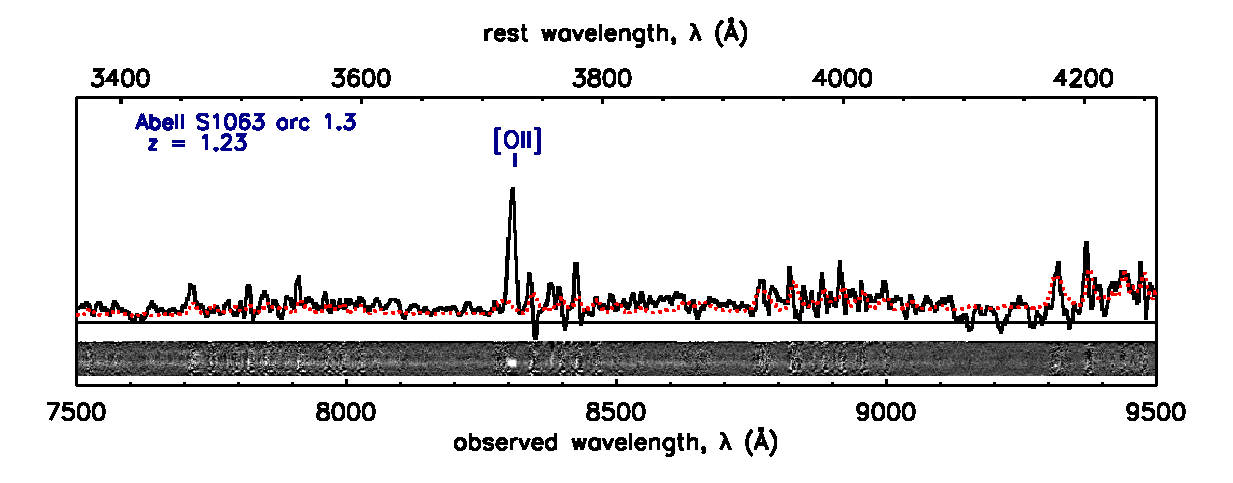
\includegraphics[width=\textwidth]{Chap2/c2f10.eps}
\caption[Abell S1063, arc 1.3 spectrum]{One-dimensional and two-dimensional spectra of Abell S1063 arc 1.3. The noise level of the one-dimensional spectrum is plotted in red.}
\label{app:fig:as1063_spec1_3}
\end{figure}

\begin{figure}[h]
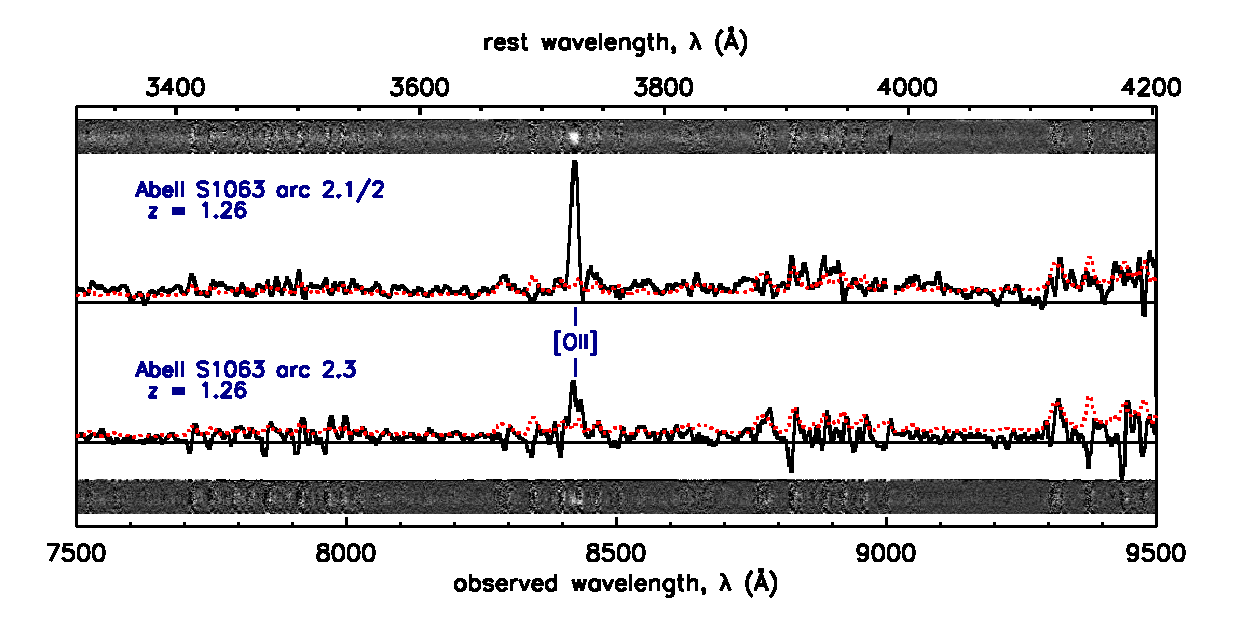
\includegraphics[width=\textwidth]{Chap2/c2f11.eps}
\caption[Abell S1063, arc 2.1/2 and 2.3 spectra]{One-dimensional and two-dimensional spectra of Abell S1063 arcs 2.1/2 (merging pair) and 2.3. The noise level of the one-dimensional spectrum is plotted in red.}
\label{app:fig:as1063_spec2}
\end{figure}

\begin{figure}[h]
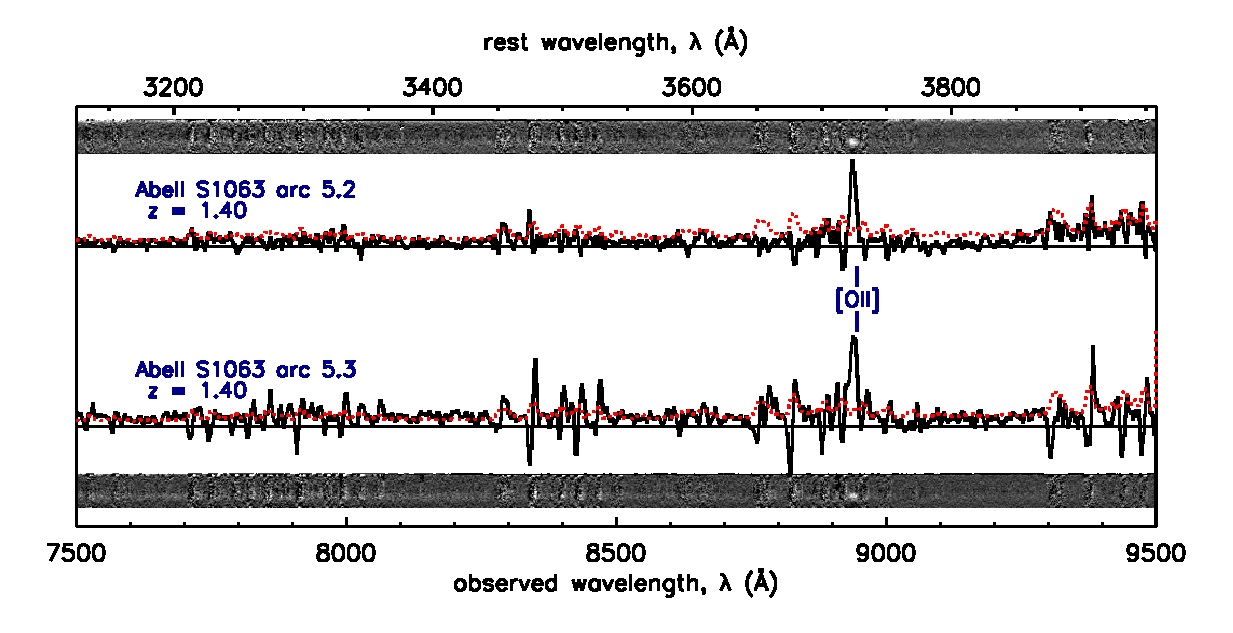
\includegraphics[width=\textwidth]{Chap2/c2f12.eps}
\caption[Abell S1063, arc 5.2 and 5.3 spectra]{One-dimensional and two-dimensional spectra of Abell S1063 arcs 5.2 and 5.3. The noise level of the one-dimensional spectrum is plotted in red.}
\label{app:fig:as1063_spec5}
\end{figure}

\newpage
\begin{figure}[h]
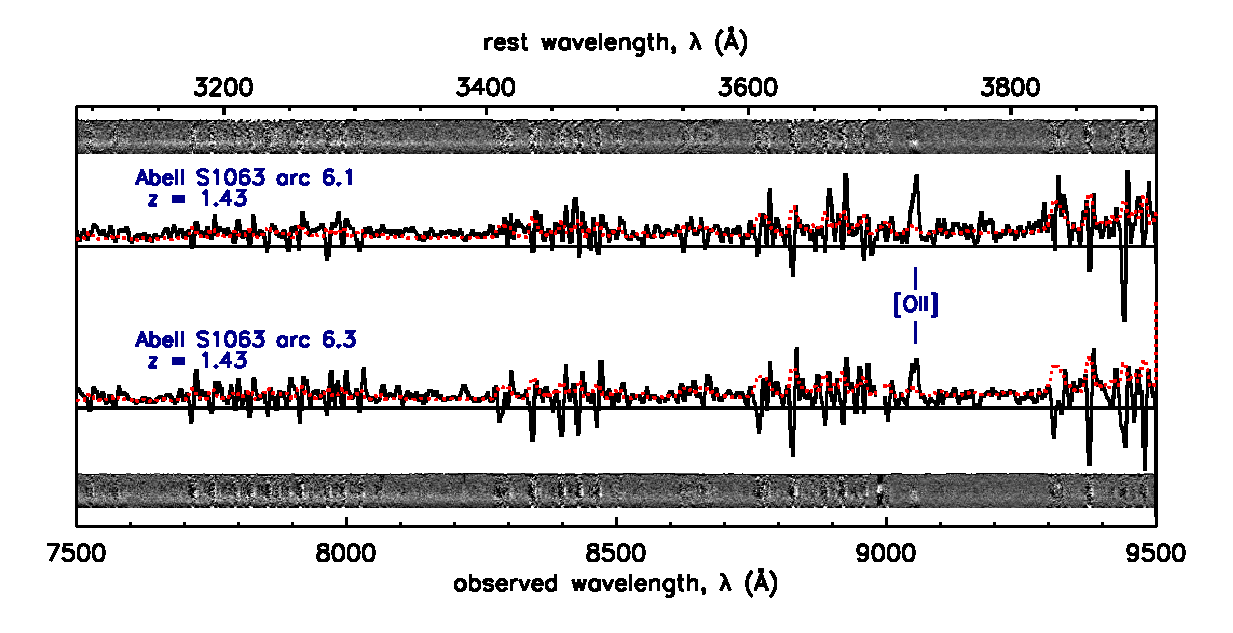
\includegraphics[width=\textwidth]{Chap2/c2f13.eps}
\caption[Abell S1063 arcs 6.1 and 6.3]{One-dimensional and two-dimensional spectra of Abell S1063 arcs 6.1 and 6.3. The noise level of the one-dimensional spectrum is plotted in red.}
\label{app:fig:as1063_spec6}
\end{figure}

\begin{figure}[h]
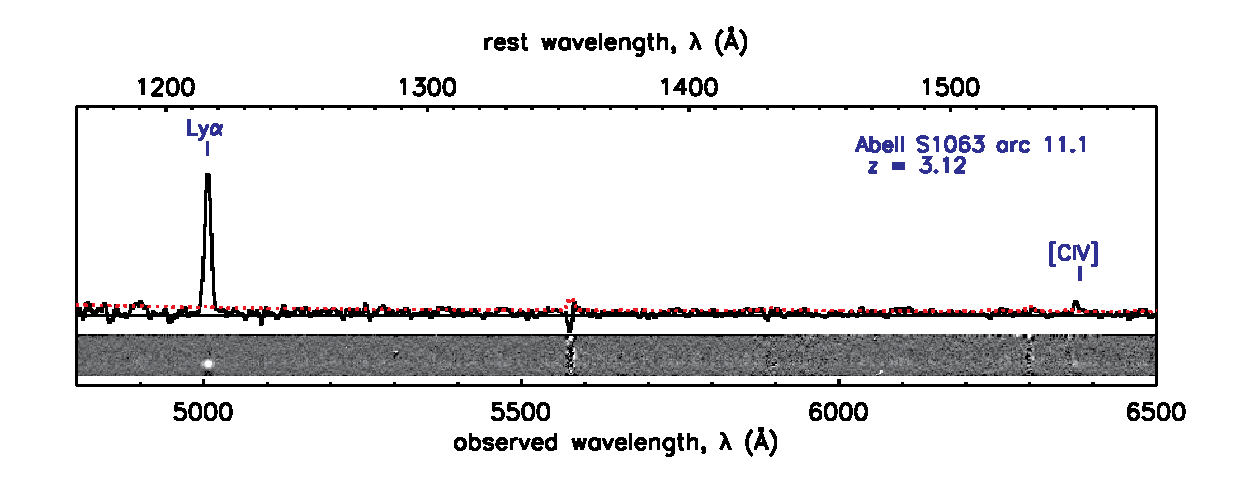
\includegraphics[width=\textwidth]{Chap2/c2f14.eps}
\caption[Abell S1063 arc 11.1 spectrum]{One-dimensional and two-dimensional spectra of Abell S1063 arc 11.1. The noise level of the one-dimensional spectrum is plotted in red.}
\label{app:fig:as1063_spec11_1}
\end{figure}

\begin{figure}[h]
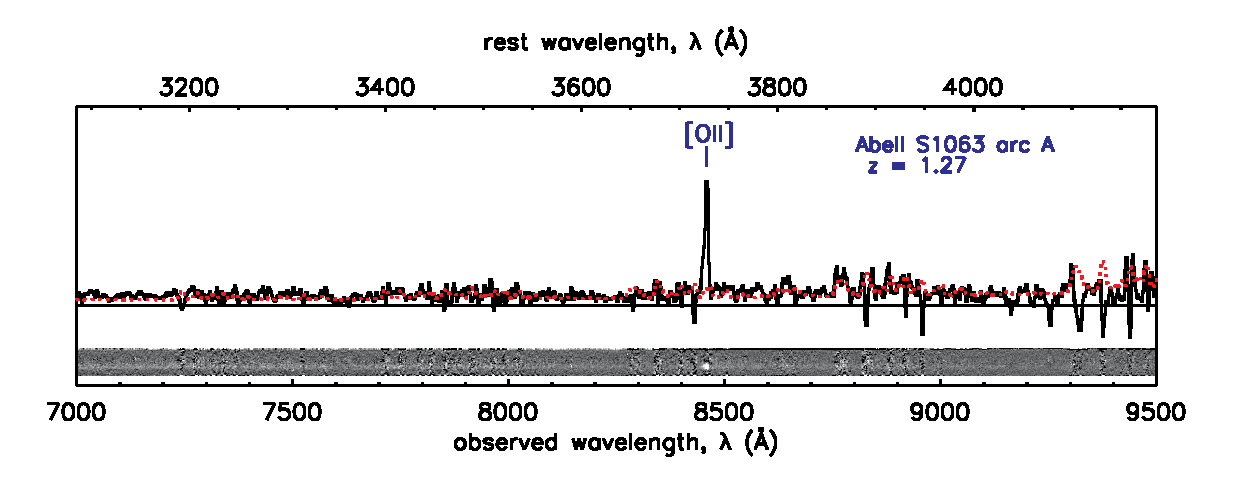
\includegraphics[width=\textwidth]{Chap2/c2f15.eps}
\caption[Abell S1063 arc A spectrum]{One-dimensional and two-dimensional spectra of Abell S1063 arc A. The noise level of the one-dimensional spectrum is plotted in red.}
\label{app:fig:as1063_specA}
\end{figure}

\begin{figure}[h]
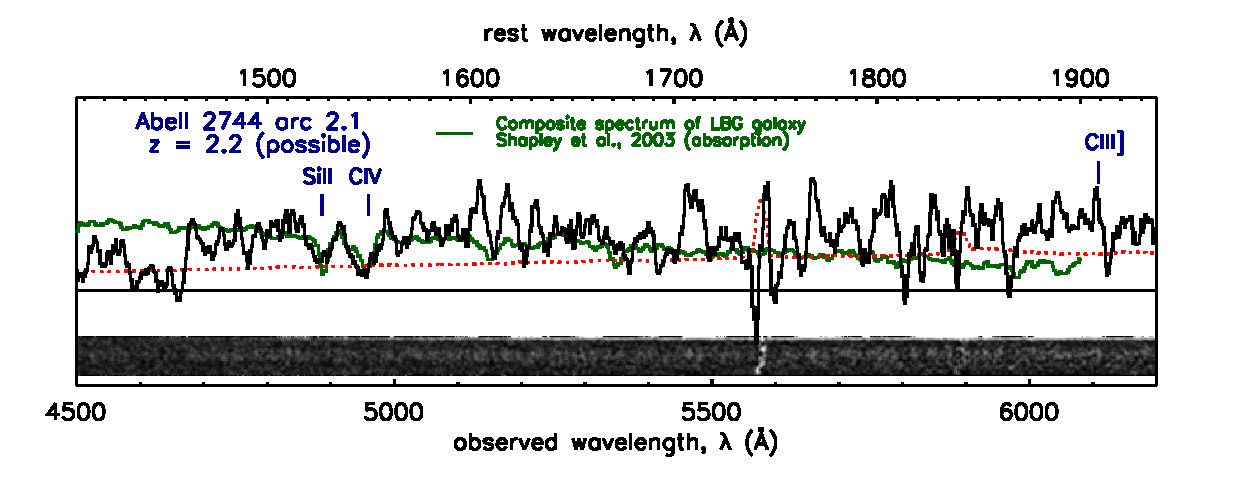
\includegraphics[width=\textwidth]{Chap2/c2f16.eps}
\caption[Abell 2744, arc 2.1 spectrum]{One-dimensional and two-dimensional spectra of Abell 2744 arc 2. The noise level of the one-dimensional spectrum is plotted in red. We over plot a composite spectrum of high-redshift ($z=3$) Lyman break galaxies with strong absorption features from \citet{Shapley:2003fk} to show similarities in spectral features as well as the Lyman break in the continuum. We find a possible solution for the redshift $z\sim2.2$ for this galaxy.}
\label{app:fig:a2744_spec2}
\end{figure}

\begin{figure}[h]
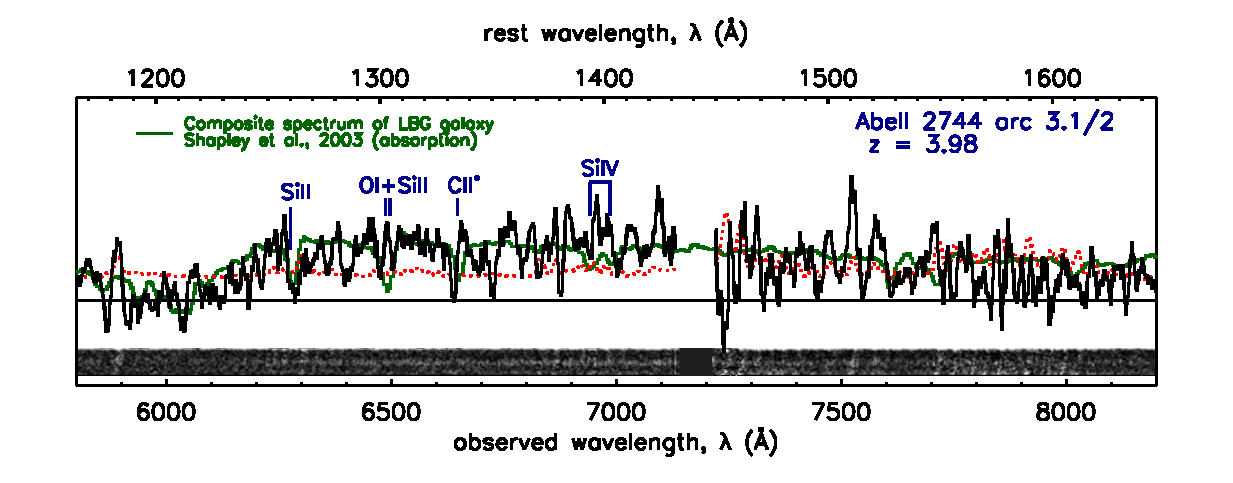
\includegraphics[width=\textwidth]{Chap2/c2f17.eps}
\caption[Abell 2744, arc 3.1/2 spectrum]{One-dimensional and two-dimensional spectra of Abell 2744 arcs 3.1/2 (merging pair). The noise level of the one-dimensional spectrum is plotted in red. We over plot a composite spectrum of high-redshift ($z=3$) Lyman break galaxies with strong absorption features from \citet{Shapley:2003fk} to show similarities in spectral features as well as the Lyman break in the continuum. This lensed arc corresponds to a star-forming galaxy at $z=3.98$.}
\label{app:fig:a2744_spec3}
\end{figure}

\newpage
\begin{figure}[h]
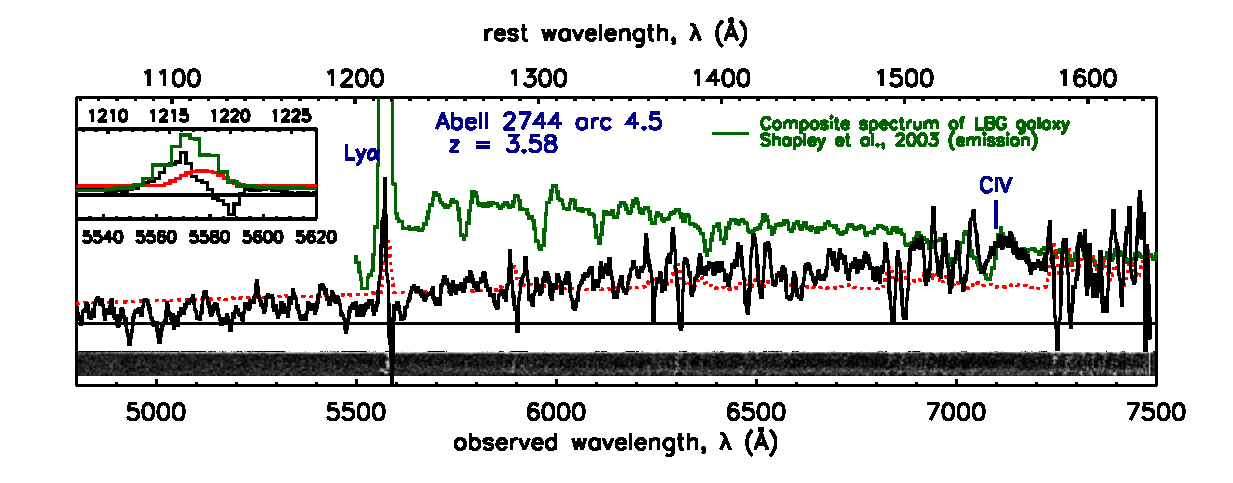
\includegraphics[width=\textwidth]{Chap2/c2f18.eps}
\caption[Abell 2744, arc 4.5 spectrum]{One-dimensional and two-dimensional spectra of Abell 2744 arc 4.5. The noise level of the one-dimensional spectrum is plotted in red. We over plot a composite spectrum of high-redshift ($z=3$) Lyman break galaxies with strong Lyman $\alpha$ emission from \citet{Shapley:2003fk} to show similarities in these spectral features as well as Lyman break in the continuum. The Ly$\alpha$ emission line lies slightly blueward of the 5577\AA\ skyline residual, as shown in the inset in the upper left. We find a likely solution of $z=3.58$ for this galaxy.}
\label{app:fig:a2744_spec4}
\end{figure}

\begin{figure}[h]
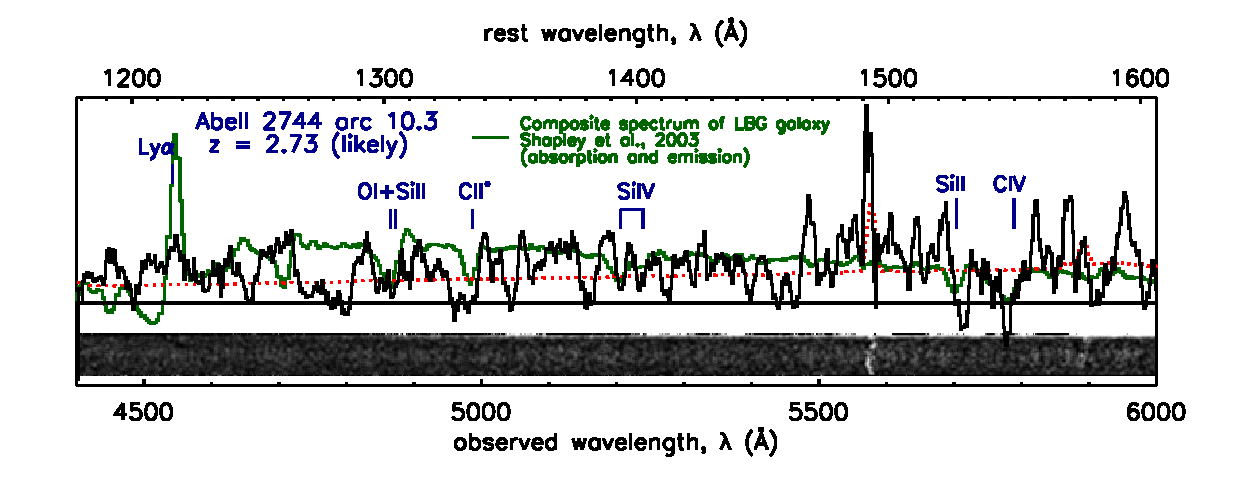
\includegraphics[width=\textwidth]{Chap2/c2f19.eps}
\caption[Abell 2744, arc 10.3 spectrum]{One-dimensional and two-dimensional spectra of Abell 2744 arc 10.3. The noise level of the one-dimensional spectrum is plotted in red. We over plot a composite spectrum of high-redshift ($z=3$) Lyman break galaxies with both strong absorption and emission features from \citet{Shapley:2003fk} to show similarities in these spectral features as well as Lyman break in the continuum. We find a possible solution for the redshift $z=2.73$ for this galaxy.}
\label{app:fig:a2744_spec10}
\end{figure}
